% Note for any github stalkers. I am currently in the process
% of learning LaTeX. I don't know what I'm doing yet. Sorry
% if my code absolutely sucks.


\documentclass{book}

\usepackage{fontspec} % used to import Calibri
\usepackage{anyfontsize} % used to adjust font size

% needed for inch and other length measurements
% to be recognized
\usepackage{calc}

% for colors and text effects as is hopefully obvious
\usepackage[dvipsnames]{xcolor}
\usepackage{soul}

% control over margins
\usepackage[margin=1in]{geometry}
\usepackage[strict]{changepage}

\usepackage{mathtools}
\usepackage{amsfonts}
\usepackage{amssymb} % originally imported to get the proof square

\usepackage{graphicx}
\graphicspath{{./140A_images/}}

\setmainfont{Calibri}
\setlength{\parindent}{0pt}
\definecolor{RawerSienna}{HTML}{945D27}

\newcommand{\hOne}{%
   \color{Black}%
   \fontsize{14}{14}\selectfont%
}
\newcommand{\hTwo}{%
   \color{MidnightBlue}%
   \fontsize{13}{13}%
}
\newcommand{\hThree}{%
   \color{PineGreen}
   \fontsize{13}{13}
}
\newcommand{\myComment}{%
   \color{RawerSienna}%
   \fontsize{12}{12}%
}
\newcommand{\teachComment}{
   \color{Orange}%
   \fontsize{12}{12}%
}
\newcommand{\exOne}{%
   \color{Purple}%
   \fontsize{14}{14}\selectfont%
}
\newcommand{\exP}{%
   \color{VioletRed}%
   \fontsize{12}{12}\selectfont%
}

\newenvironment{myIndent}{%
   \begin{adjustwidth}{2.5em}{0em}%
}{%
   \end{adjustwidth}%
}

\newcommand{\udefine}[1]{%
   \setulcolor{Red}%
   \setul{0.1ex}{0.15ex}%
   \ul{#1}%
}

\newcommand{\uuline}[1]{%
   \setulcolor{Black}%
   \setul{0.15ex}{0.1ex}\ul{#1}%
   \setul{0.50ex}{0.1ex}\llap{\ul{#1}}%
}

\newcounter{LectureNumber}
\newcommand*{\markLecture}[1]{%
   \stepcounter{LectureNumber}%
   {\huge \color{Black} \textbf{Lecture \theLectureNumber: #1} \newline}%
}

\newcommand{\pprime}{\prime\prime}

\newcounter{PropNumber}
\newcommand{\propCount}{%
   \stepcounter{PropNumber}%
   \thePropNumber%
}

\newcommand{\mySep}[1]{%
   {\noindent\color{#1}{\rule{16cm}{1mm}}}\\%
}


\title{Math 140A Lecture Notes (Professor: Brandon Seward)}
\author{Isabelle Mills}


\begin{document}
   \maketitle

   \markLecture{1/8/2024}

   \hOne
   An \udefine{order} on a set $S$, typically denoted as $<$, is
   a binary relation satisfying:
   \begin{enumerate}
      \item $\forall x, y \in S$, exactly one of the following is true:
      \begin{itemize}
         \item $x<y$ \item $x=y$ \item $y<x$
      \end{itemize}

      \item given $x, y, z \in S$, we have that $x<y<z\Rightarrow x<z$
   \end{enumerate}
   \hfill \bigbreak

   As a shorthand, we will specify that
   \begin{itemize}
      \item $x>y \Leftrightarrow y<x$
      \item $x\leq y \Leftrightarrow x<y \text{ or } x=y$
      \item $x\geq y \Leftrightarrow x>y \text{ or } x=y$
   \end{itemize}

   An \udefine{ordered set} is a set with a specified ordering. Let
   $S$ be an ordered set and $E$ be a nonempty subset of $S$. 

   \hTwo
   \begin{myIndent}
   \begin{itemize}
      \item If $b \in S$ has the property that $\forall x \in E, \hspace{0.25em}
      x \leq b$, then we call $b$ an\\ \udefine{upperbound} to $E$ and 
      say that $E$ is \udefine{bounded above} by $b$.
      \hfill \bigbreak
      
      \item if $b \in S$ has the property that $\forall x \in E, 
      \hspace{0.25em} x \geq b$, then we call $b$ an 
      \udefine{lower bound} to $E$ and say that $E$ is 
      \udefine{bounded below} by $b$.
      \hfill \bigbreak
   
      \item We call $\beta \in S$ the \udefine{least upperbound} to $E$ if
      $\beta$ is an upper bound to $E$ and $\beta$ is the least of all
      upperbounds to $E$. In this case, we also commonly call $\beta$ 
      the \udefine{supremum} of $E$ and denote it as $\sup{E}$.
      \hfill \bigbreak
   
      \item We call $\beta \in S$ the \udefine{greatest lower bound} to $E$ if
      $\beta$ is an lower bound to $E$ and $\beta$ is the greatest of all
      lower bounds to $E$. In this case, we also commonly call $\beta$ 
      the \udefine{infimum} of $E$ and denote it as $\inf{E}$.
      \hfill \bigbreak

      \item We call $e \in E$ the \udefine{maximum} of E if $\forall 
      x \in E, \hspace{0.25em} x \leq e$
      \hfill \bigbreak

      \item We call $e \in E$ the \udefine{minimum} of E if $\forall 
      x \in E, \hspace{0.25em} x \geq e$
      \hfill \bigbreak
   \end{itemize}
   \end{myIndent}

   \hOne
   \uuline{Fact}: For an ordered set $S$ and nonempty $E\subseteq S$,
   either:
   \begin{itemize}
      \item neither $\max{E}$ nor $\sup{E}$ exists
      \item $\sup{E}$ exists but $\max{E}$ does not exist
      \item $\max{E}$ exists and $\sup{E}=\max{E}$
   \end{itemize}

   \pagebreak
   \exOne
   Using $\mathbb{Q}$ as our ordered set...
   \begin{itemize}
      \item For $E = \{q \in \mathbb{Q} \mid 0<q<1\}$,
      $\max{E}$ does not exist but $\sup{E}$ exists and equals $1$.
      \exP
      \begin{myIndent}
         To understand why, note that the set of all upper bounds
         of $E$ is equal to\\ $\{q \in \mathbb{Q} \mid q \geq 1\}$ and 
         $1$ is obviously the smallest element of that set. Thus, $1$
         is the supremum of $E$. However, $1 \notin E$. Thus, if
         $\max{E}$ did exist, it would have to not equal $1$. But that
         would contradict $1$ being the least greatest bound.
      \end{myIndent}
      \hfill \bigbreak

      \exOne
      \item For $E = \{q \in \mathbb{Q} \mid 0<q \leq 1\}$,
      $\max{E}$ and $\sup{E}$ exist and they both are equal to $1$
      \exP
      \begin{myIndent}
         The reasoning for this is similar to that for the previous set.
      \end{myIndent}
      \hfill \bigbreak
      
      \exOne
      \item For $E = \{q \in \mathbb{Q} \mid q^2 < 2\}$, neither
      $\max{E}$ and $\sup{E}$ exist.
      \exP
      \begin{myIndent}
         To prove this, we can show that there exists a function $f: 
         \mathbb{Q}^+ \rightarrow \mathbb{Q}^+$ such that
         $\forall q \in \mathbb{Q}^+$, we have that $q^2 < 2
         \Rightarrow q^2 < (f(q))^2 < 2 \text{ and } 2 < q^2
         \Rightarrow 2 < (f(q))^2 < q^2$. Thus, we can show that
         the set of upper bounds to $E$ has no minimum element (meaning
         $\sup{E}$ is undefined) and $E$ itself has no maximum element.
         \hfill \bigbreak


         Now instead of being like Rudin and simply providing the desired
         function, I want to present how one may come up with a function 
         that works for this proof themselves.
         \hfill \bigbreak

         Firstly, note that for the following reasons, we know our 
         desired function must be a rational function:
         \begin{itemize}
            \item[$\diamond$] $\forall q \in \mathbb{Q}, \hspace{0.25em} 
            f(q) \in \mathbb{Q}$. Based on this, we can't use any radicals,
            trig functions, logarithms, or exponentials in our desired
            function. \hfill \bigbreak

            \item[$\diamond$] $q^2 > 2 \Rightarrow f(q) < q$. In other
            words, $f$ needs to grow slower than a linear function. Thus,
            we can rule out the possibility of $f$ being a polynomial.
            \hfill \bigbreak

            \item[$\diamond$] If we wanted $f$ to be a linear function,
            it would have to have the form\\ $f(q) = \alpha(q - \sqrt{2})
            + \sqrt{2}$ where $\alpha$ is some constant. This is
            because when $q^2 = 2, \hspace{0.25em} f(q) = q$. However, there
            is no value one can set $\alpha$ to which both eliminates the
            presence of irrational numbers in that function while
            simultaneously making $f(q) \neq q$ when $q^2 \neq 2$. So
            no linear function can possibly work for this proof.
            \hfill \bigbreak
         \end{itemize}

         Having narrowed our search, let's now pick some convenient
         properties we would wish our proof function to have. Specifically,
         let's force $f$ to be constantly increasing, have a $y$-intercept
         of $1$, and approach a horizontal asymptote of $y = 2$. Doing this,
         we can now say that an acceptable function will have the following
         form where $\alpha$ is an unknown constant:
         \[f(q) = 1 + \frac{q}{q + \alpha}\]
         
         And finally, we can solve for $\alpha$ using the following system
         of equations:
         \[\begin{matrix}
            (1 + \frac{q}{q + \alpha})^2 = 2 \\
            \\
            1 + \frac{q}{q + \alpha} = q
         \end{matrix}\]

         Now here's where a graphing calculator like Desmos can be very
         useful. Instead of painstakely having to solve for $\alpha$,
         we can use a graphing calculator to approximate the value of
         $\alpha$ that satisfies our system of equations.
         \begin{center}
         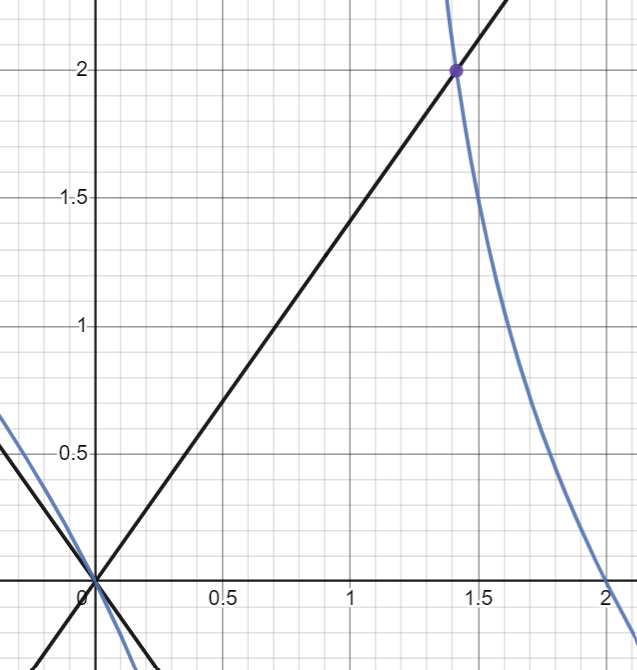
\includegraphics[scale=0.75]{Finding_Equation_Demonstration_1.png}
         \end{center}

         Based on the graph above, it looks like $f(q) = 1 +
         \frac{q}{q + 2}$ will work for our proof. And sure enough 
         it does. Furthermore, we can verify that the function we came
         up with is equivalent to that which Rudin presents.
      \end{myIndent}
   \end{itemize}

   \mySep{Purple}
   \hOne\hfill \break
   We say an ordered set $S$ has the \udefine{least upper bound
   property} if and only if when $E \subseteq S$ is nonempty and 
   bounded above, then the supremum of $E$ exists in $S$. Additionally, 
   we say an ordered set $S$ has the \udefine{greatest lower bound 
   property} if and only if when $E \subseteq S$ is nonempty and 
   bounded below, then the infimum of $E$ exists in $S$.
   
   \begin{myIndent}\begin{myIndent}\begin{myIndent}
   \begin{myIndent}\begin{myIndent}
      \teachComment
      When we define the set of real numbers, this will be one of the
      fundamental properties of that set. \hfill \bigbreak
   \end{myIndent}\end{myIndent}\end{myIndent}
   \end{myIndent}\end{myIndent}

   \markLecture{1/10/2024}
   \begin{myIndent}
      \hTwo
      Proposition \propCount: $S$ has the least upper bound property if
      and only if $S$ has the greatest lower bound property.
      
      \hThree
      \begin{myIndent}
         Proof: Let's say we have an ordered set $S$
         \hfill \bigbreak

         First, //waiting for class next wednesday... It's late and I want
         to go to bed...

      \end{myIndent}

   \end{myIndent}


\end{document}